\section{类脑注意力机制}
\subsection{平滑跟踪大脑皮层通路解剖对齐的视觉跟踪模型}


\begin{frame}{DNN 和带有BTS的神经解剖学对齐之间的协同设计}
	\begin{figure}[!t]
		\centering
		\includegraphics[width=4.5in]{../figures/C2Fig/introduction.pdf}
		%		\caption{DNN 和带有BTS的神经解剖学对齐之间的协同设计}
		\label{ch2_introduction}
	\end{figure}
\end{frame}


\begin{frame}{类脑视觉目标跟踪的网络架构}
	\begin{figure}[!t]
		\centering
		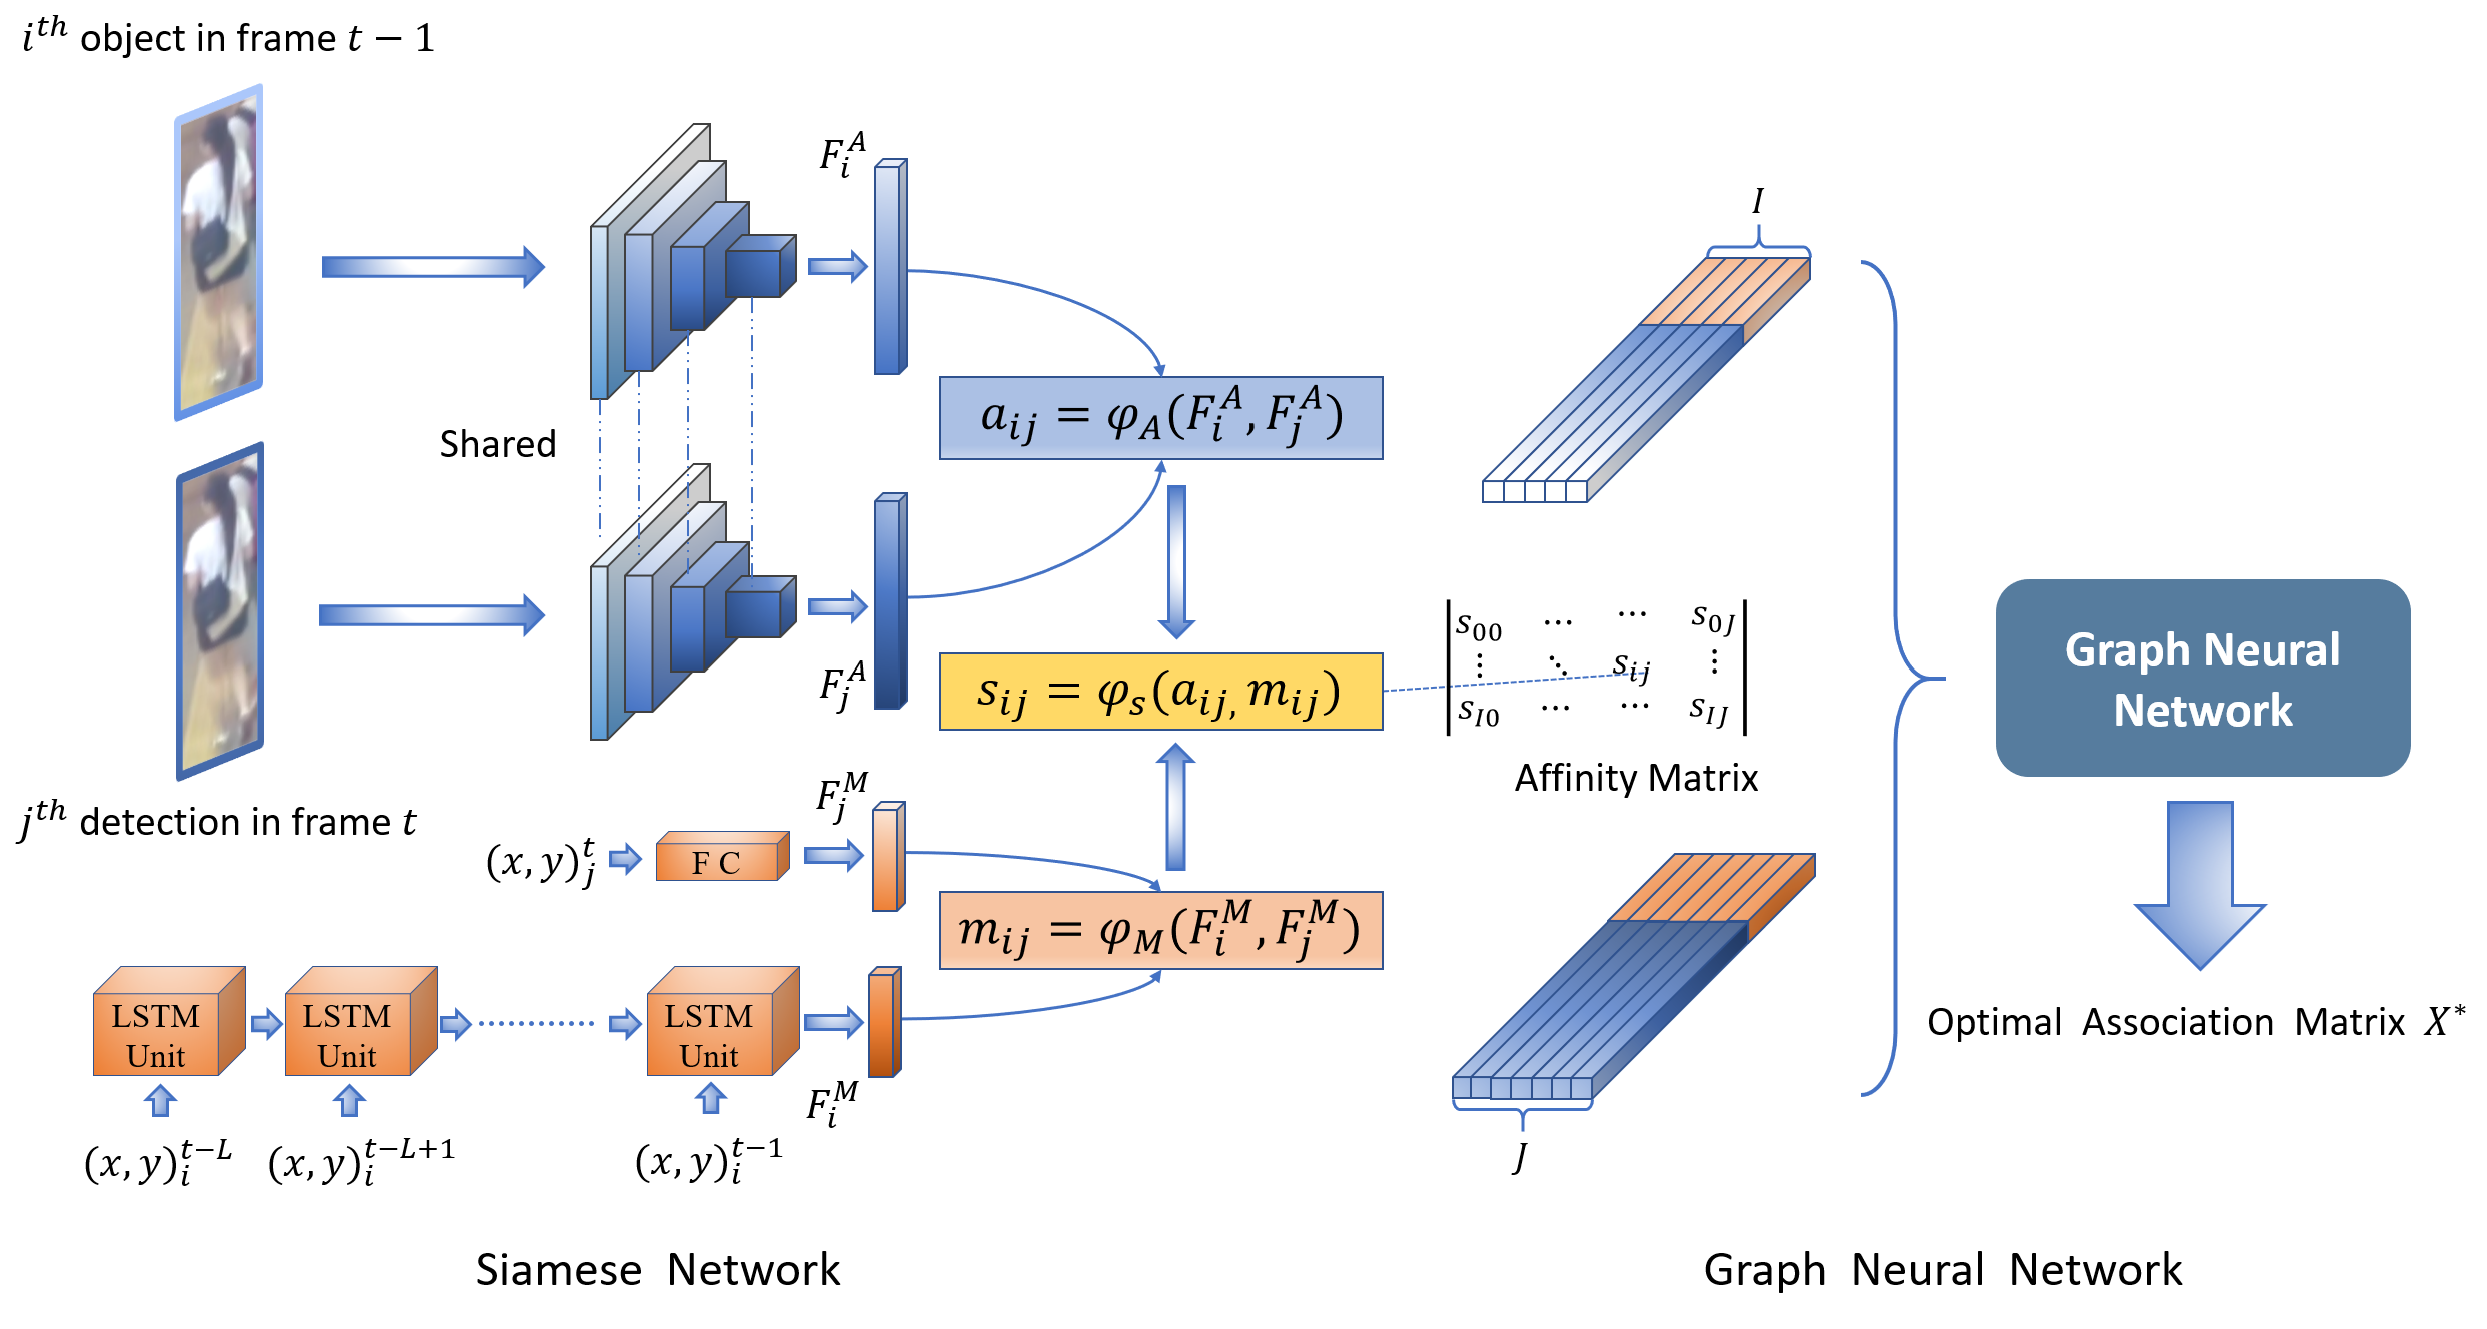
\includegraphics[width=4.5in]{../figures/C2Fig/pipeline.pdf}
		%		\caption{类脑视觉目标跟踪的网络架构}
		\label{ch2_pipeline}
	\end{figure}
\end{frame}


\begin{frame}{大脑——神经网络中各个模块的建模}
	\begin{columns}[T] % align columns
		\begin{column}<0->{.40\textwidth}
			\begin{block}{运动信号处理}
				视网膜
				\begin{itemize}
					\item<0-> $ f_t = M_t^y F_t (M_t^x)^T $
				\end{itemize}
				
				腹侧通路
				\begin{itemize}
					\item<0-> 卷积神经网络
				\end{itemize}
				
				背侧通路
				\begin{itemize}
					\item<0-> $ \left\{ \phi _t ^i \right\}_{i=1}^N = \text{FC}(\alpha_t) $
				\end{itemize}
				
				腹/背侧整合
				\begin{itemize}
					\item<0-> $ m_t = \text{FC}(conc(v_t \odot d_t)) $
				\end{itemize}
			\end{block}
			
		\end{column}
		\hfill%
		
		\begin{column}<0->{.65\textwidth}
			\begin{figure}[!t]
				\centering
				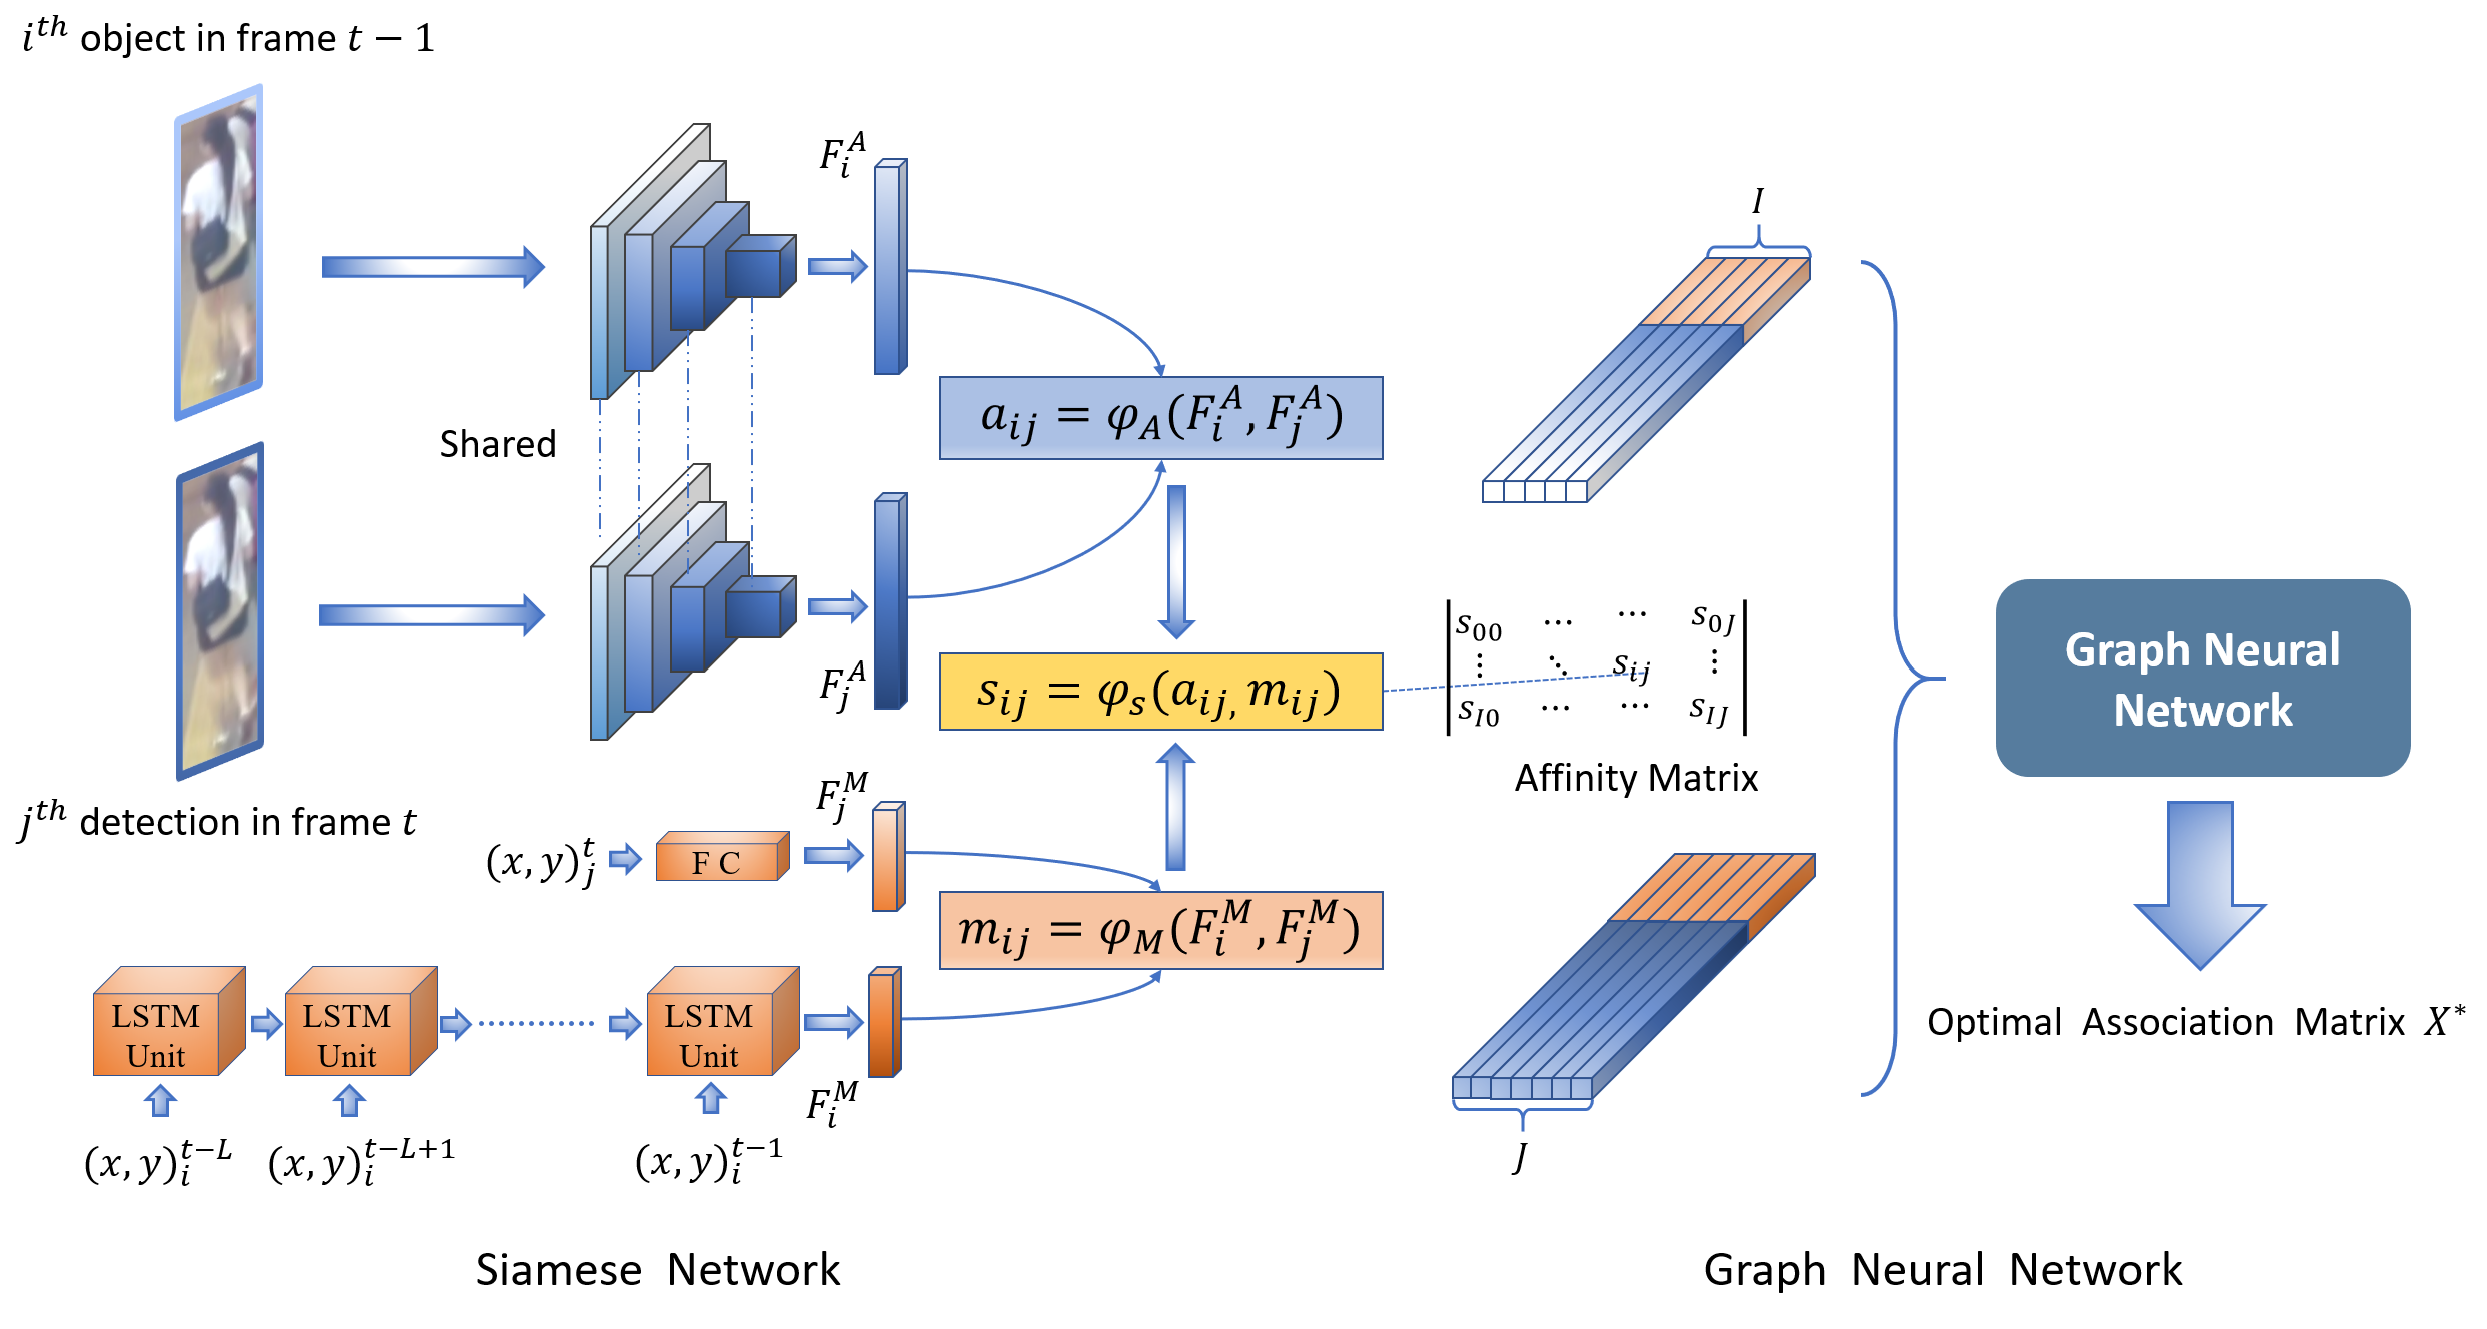
\includegraphics[width=2.8in]{../figures/C2Fig/pipeline.pdf}
				%			\caption{类脑视觉目标跟踪的网络架构}
			\end{figure}
		\end{column}%
	\end{columns}
	
\end{frame}


\begin{frame}{大脑——神经网络中各个模块的建模}
	\begin{columns}[T] % align columns
		\begin{column}<0->{.40\textwidth}
			
			\begin{block}{运动信号转化}
				额叶视区
				\begin{itemize}
					\item<0-> $ h_t, o_t = \text{LSTM}(h_{t-1}, m_t) $
				\end{itemize}
				
				脑干和小脑
				\begin{itemize}
					\item<0-> $ \Delta p_t, \Delta a_{t+1}, \alpha_{t+1} = \text{FC}(conc(d_t), o_t) $
					\item<0-> $ a_{t+1} = a_t + tanh(c) \Delta a_{t+1} $
					\item<0-> $ p_t = a_t + \Delta p_t $
					\item<0-> $ \Delta p_t = \Delta p $
				\end{itemize}
			\end{block}
			
		\end{column}
		\hfill%
		
		\begin{column}<0->{.65\textwidth}
			\begin{figure}[!t]
				\centering
				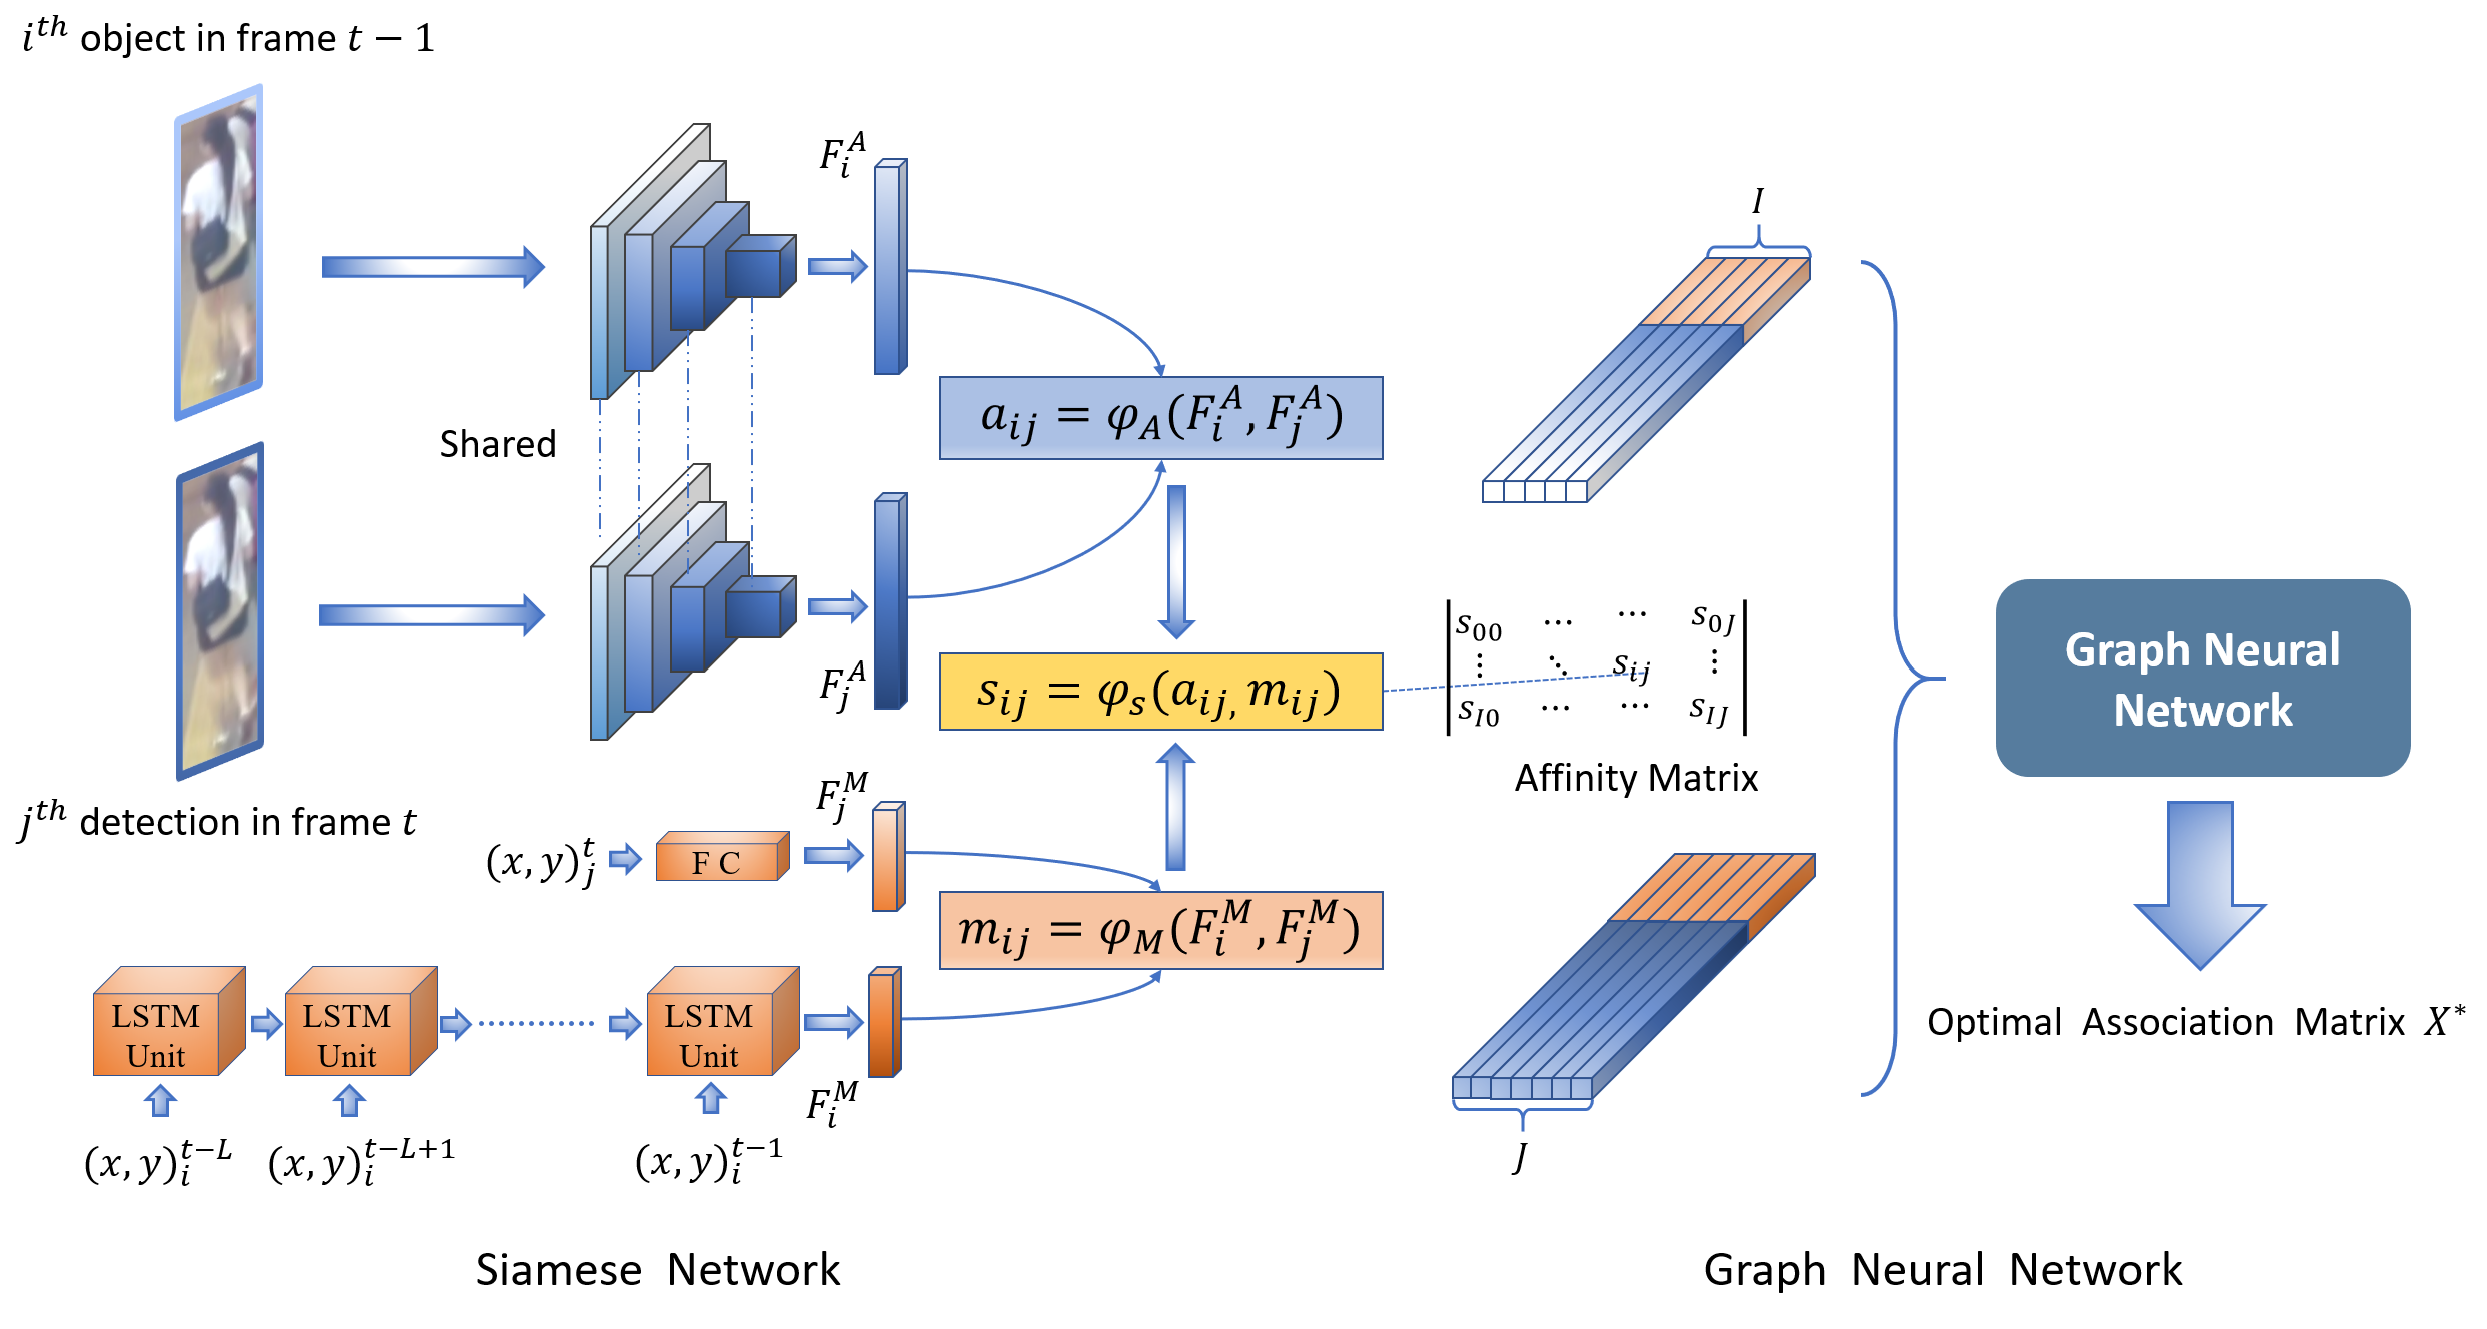
\includegraphics[width=2.8in]{../figures/C2Fig/pipeline.pdf}
				%				\caption{类脑视觉目标跟踪的网络架构}
			\end{figure}
		\end{column}%
	\end{columns}
	
\end{frame}


\begin{frame}{损失函数设计}
	\begin{columns}[T] % align columns
		\begin{column}<0->{.40\textwidth}
			\begin{block}{}
				跟踪损失
				\begin{itemize}
					\item<0-> $ L_t = -\log(\mbox{IoU} ( \frac{p_t \cap \hat{p}_t}{p_t \cup \hat{p}_t} )) $
				\end{itemize}
				
				背侧通路
				\begin{itemize}
					\item<0-> $ L_d = -\log (\frac{a_t \cap p_t}{p_t}) - \log (1 - \frac{a_t \cap F_t}{a_t \cup F_t}) $
				\end{itemize}
				
				腹侧流损失
				\begin{itemize}
					\item<0-> $ L_v = - r(a_t, p_t) \log(d_t) $
				\end{itemize}
				
				辅助损失
				\begin{itemize}
					\item<0-> $ L_a = 
					\frac{1}{2} \left\vert \left\vert \theta \right\vert \right\vert _2 ^2 + 
					\frac{1}{2} \left\vert \left\vert \phi_t \right\vert \right\vert _2 ^2
					- \sum_{i} \log (\lambda_i^{-1}) $
				\end{itemize}
			\end{block}
		\end{column}
		\hfill%
		
		\begin{column}<0->{.65\textwidth}
			\begin{figure}[!t]
				\centering
				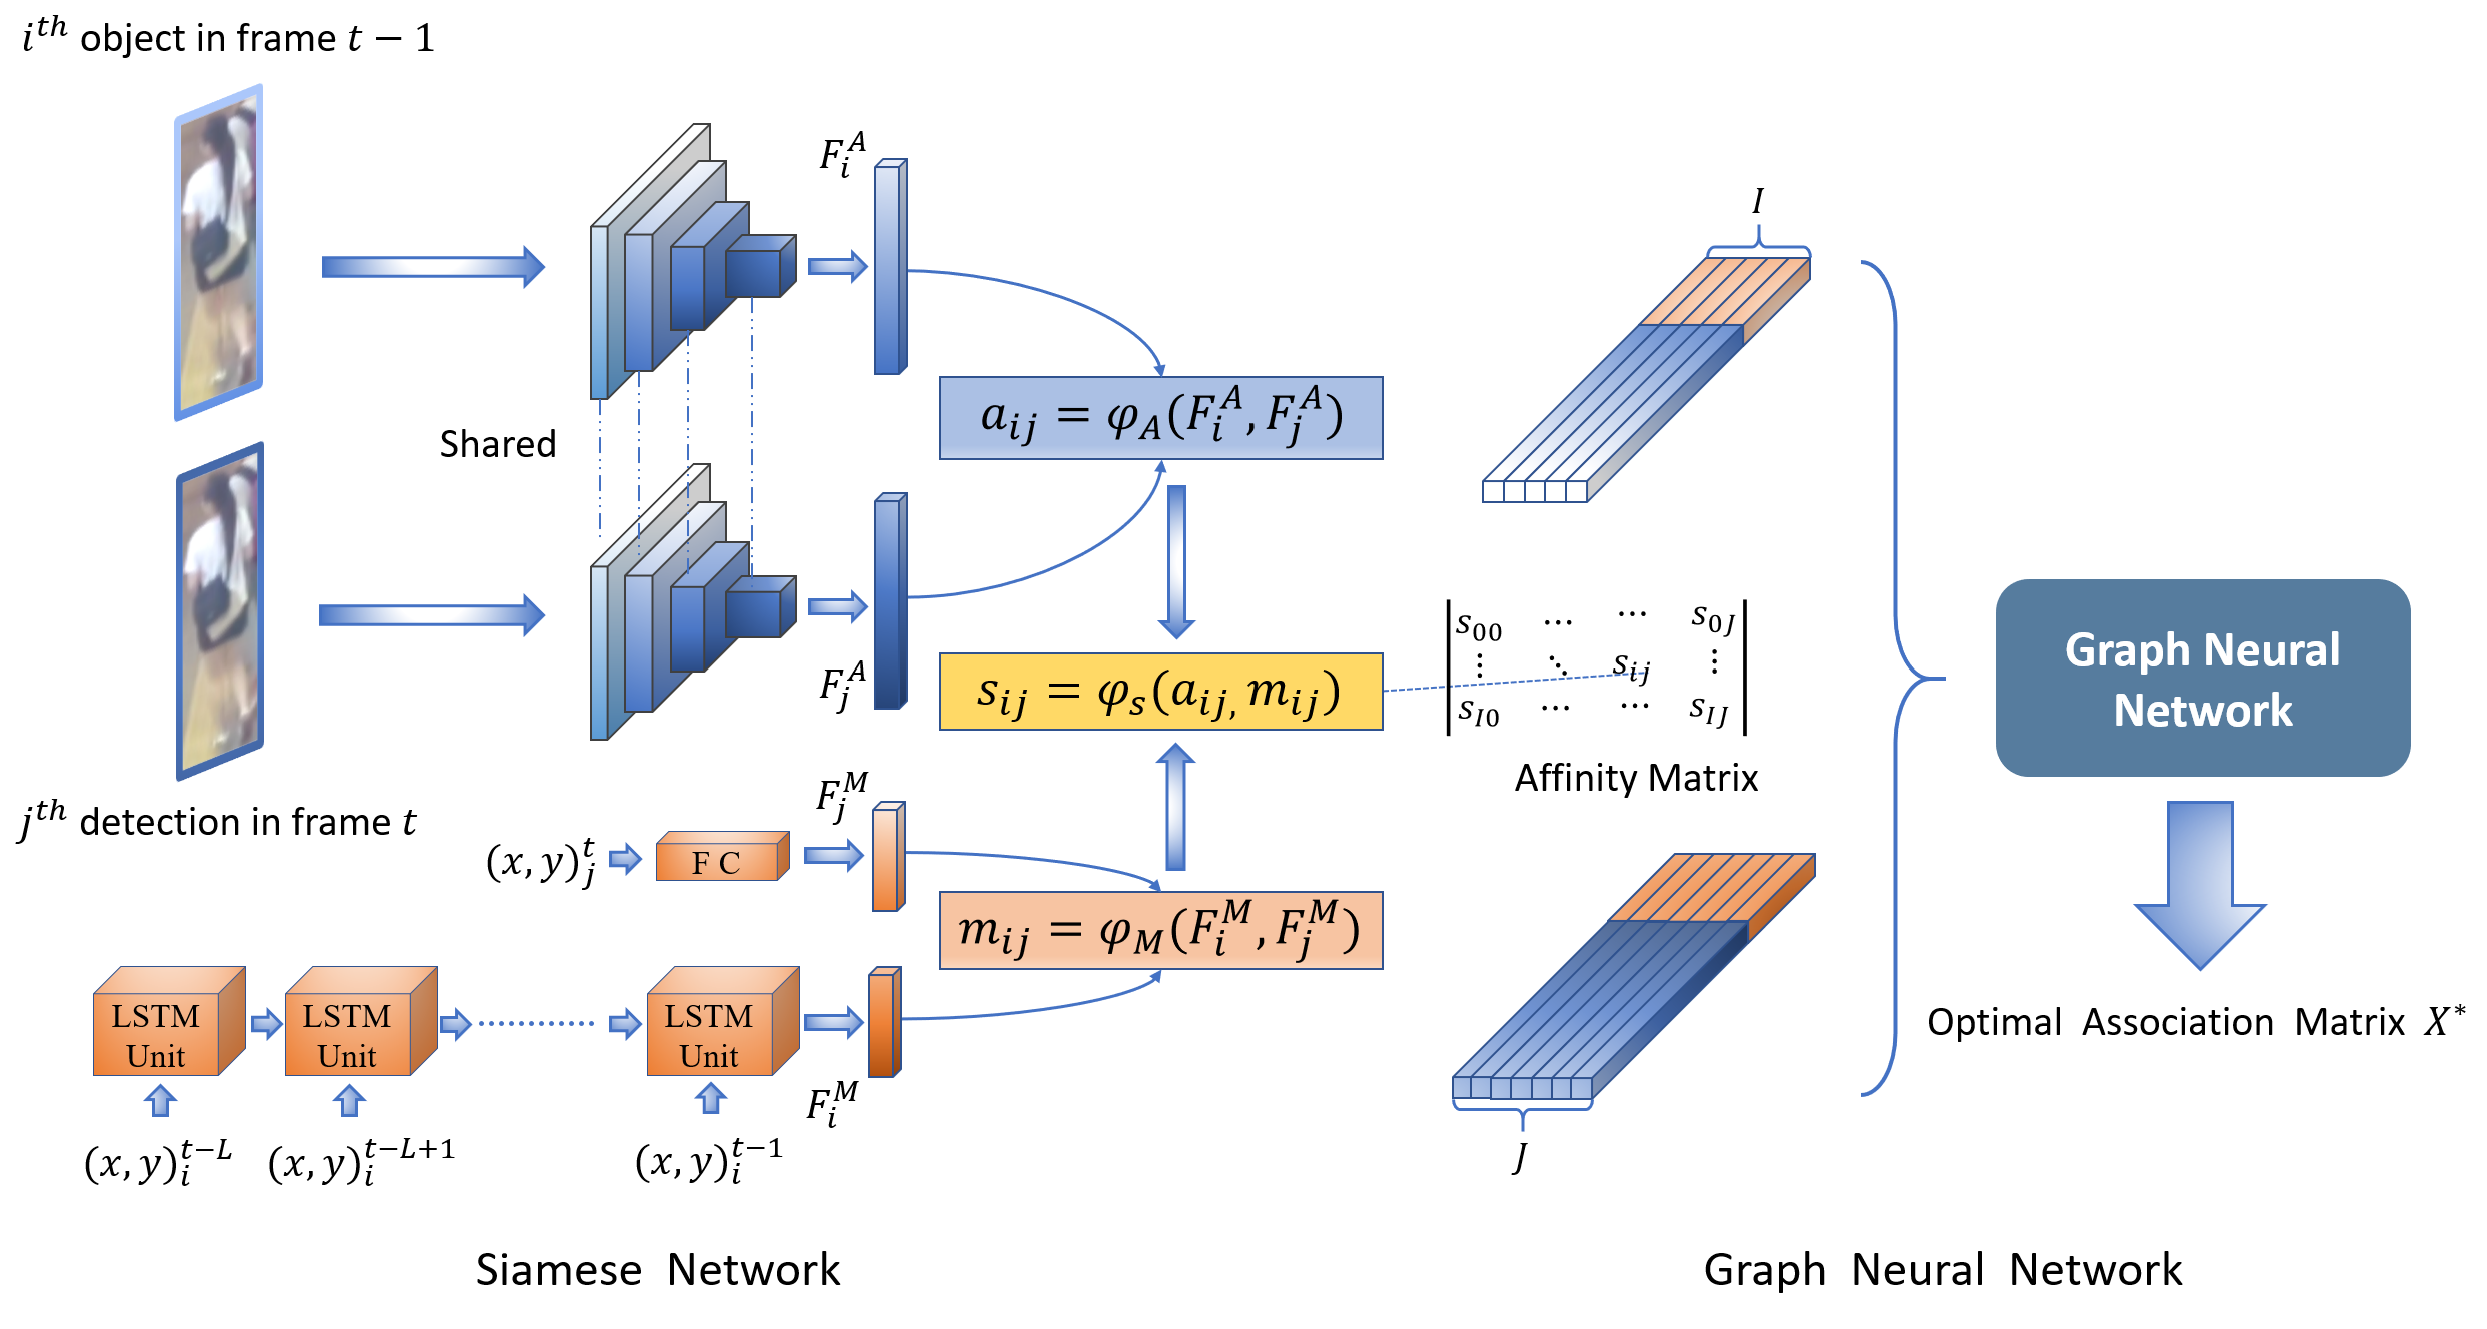
\includegraphics[width=2.8in]{../figures/C2Fig/pipeline.pdf}
				%				\caption{类脑视觉目标跟踪的网络架构}
			\end{figure}
		\end{column}%
	\end{columns}
	
\end{frame}


\begin{frame}{大脑数据分析}
	\begin{block}{\textbf{基本思路}}
		\begin{itemize}
			\item<0-> 为了比较DNN 的视觉目标跟踪和人脑平滑跟踪的相似性,首先需要从各种眼球运动中提取平滑跟踪,然后选择相应的大脑区域和激活用于相似性计算。
		\end{itemize}
	\end{block}
	
	\begin{block}{\textbf{实现步骤}}
		\begin{enumerate}
			\item<0-> 视频刺激的运动估计
			\item<0-> 平稳跟踪样本的提取
			\item<0-> 回归变量建模
			\item<0-> 核磁共振数据分析
		\end{enumerate}
	\end{block}
\end{frame}


\begin{frame}{评价指标:类脑跟踪分数}
	为了在统一指标上评估BTN,该指标计算了眼动行为预测性指标和皮层神经皮层
	预测性指标的平均值,眼动行为预测性表示为:
	\[  s_b=\frac{area(S_{roi}^a \cap S_{roi}^b) }  { area(S_{roi}^a \cup S_{roi}^b) }   \]
	皮层神经预测性表示为:
	\[  s_r=\frac{\sum_{i=1}^{n} (y_i-\bar{y}) (y_i^\prime - \bar{y}^\prime) }{\sqrt{\sum_{i=1}^{n} (y_i - \bar{y})^2 (y_i^\prime - \bar{y}^\prime)^2 }}  \]
	总分数 $s_{t}$ 是两个分数的平均值:
	\[  s_{t} = \frac{s_b + s_r}{2}  \]
	\begin{center}
		\textcolor{mymauve}{BTS 的设计没有在各个分数大小上进行归一化,因为归一化可能会惩罚方差较小的分数。}
	\end{center}
\end{frame}


\begin{frame}{实验结果}
	\begin{columns}[T] % align columns
		\begin{column}<0->{.40\textwidth}
			\begin{figure}[!t]
				\centering
				\includegraphics[width=2.0in]{../figures/C2Fig/comp_sim.pdf}
				\caption{BTN捕获的MT/MST神经响应}
			\end{figure}
		\end{column}
		\hfill%
		
		\begin{column}<0->{.65\textwidth}
			\begin{figure}[!t]
				\centering
				\includegraphics[width=2.0in]{../figures/C2Fig/structure_analysis.pdf}
				\caption{BTN架构分析}
			\end{figure}
		\end{column}%
	\end{columns}
	
\end{frame}

\begin{frame}{实验效果可视化}
	\begin{figure}[!t]
		\centering
		\includegraphics[width=4.5in]{../figures/C2Fig/tracking.pdf}
		\caption{在Tracking-Gump 数据集上跟踪测试所提出模型效果的示例}
	\end{figure}
\end{frame}